
"Sensorimotor" indicates the involvement of both sensory and motor functions. The ability to execute sensorimotor tasks well is crucial for performance in athletic activity. Moreover, there is an abundance of research suggesting the connection between sensorimotor performance and injury. Therefore, great effort is directed to understanding these skills. In this section we will briefly review the literature intersecting sensorimotor performance and injury. In particular we will also introduce a method that involves an action known as the single leg drop jump (SLDJ) which is frequently used to measure sensorimotor performance. 

SLDJ is a unilateral horizontal drop jump, in other words the subject hops off an elevated platform of usually 30cm. It has shown to be more reliable, in means of reproducibility, than other sensorimotor performance tasks and is known to show similarities to the bilateral drop jump which is used is many areas including athlete assessment, performance monitoring, talent identification and rehabilitation \cite{Stalbom2007ReliabilityReport}.

\begin{figure}[hb]
	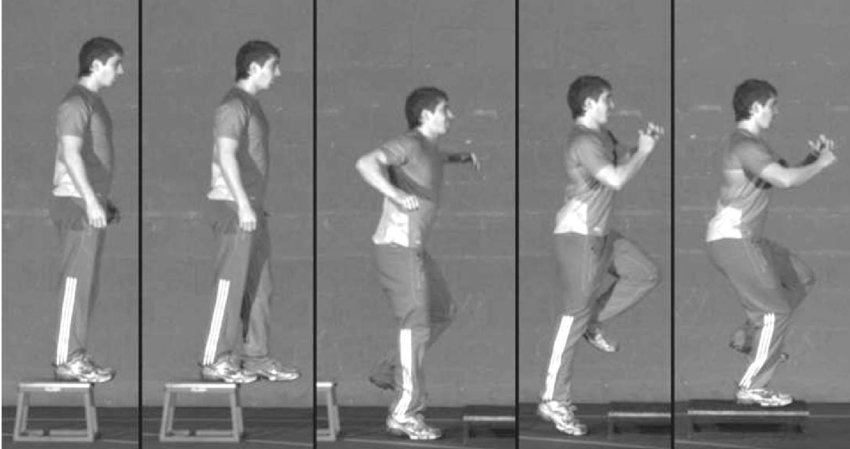
\includegraphics[width = \linewidth]{images/jump/sldj.png}
	\caption{Single leg drop jump\cite{Wild2011ABiomechanical}.}
	\label{homo}
\end{figure}


\newpage
%===============================
% * New page
%===============================

\subsection{Ground Reaction Forces}

There are largely two methods of measuring a SLDJ. The first is by measuring the ground reactions forces (GRFs) using a special measurement device known as a force plate. Several indicators such as Time to stabilization (TTS) \cite{Fransz2014HowTask}, dynamic postural stability index (DPSI) \cite{Huurnink2019TheStudy} center of pressure (COP) \cite{Fransz2014HowTask} are then calculated and are assessed. A number of studies show that TTS, DPSI, COP can be used to differente participants between chronic ankle instability (CAI), functional ankle instability (FAI), anterior cruciate ligament etc \cite{WIKSTROM2005DetectionInstability}. Yet, to date, the interrelations among TTS, DPSI, and other indicators are largely unknown \cite{Huurnink2019TheStudy}. 

It is important to note that there are multiple variations to calculate the above methods due to the possibility of different sample rate, filter settings or trial length. Such variances can cause a difference on outcome values that may lead to contradictory results \cite{Fransz2015TimeValues}. This makes it difficult to determine whether one can correclty infer probability of injury using GRF measurements.

\subsection{Pose Characteristics}
The second method of measurement of SLDJ is the measurement of pose characteristics using either manual notation or automated motion capture. In most cases captured data is then analysed manually, without the use of machine learning techniques. It has been shown that women have a greater valgus knee angle at time of initial contact then men performing a SLDJ \cite{Russell2006SexJump}. However, due to the high-dimensional and multivariate nature of this data, there only a handful of research focusing on the measurement of pose characteristics. In this paper we aim to overcome this difficulty using subspace based classifiers and introduce a method that can be used to conduct classification using motion capture data.

